\documentclass{article}
\usepackage{graphicx}

\begin{document}

\title{Sentiment Analysis of Trump's Tweets Before Election}
\author{Zhenmin Li}

\maketitle

\begin{abstract}
This project tried to solve the data source problem of project 1.
\end{abstract}

\section{Content}

As I mentioned in project 1, I used the dataset from Kaggle and the size is not enough for analysis. In this project I use tweepy to parse tweets from Trump. The size is stil limited becasue I use a free API. A paid one can do it better with the same script.
\\ \hspace*{\fill} \\ 
This project is a seperate one because I don't need rscripts from project 1. I did some sentiment analysis different from project 1 and generated a line chart.
\\ \hspace*{\fill} \\ 
In this project I use a different sentiment analysis method in textblob. This product polarity and subject as two elements.

\begin{figure}[h]
    \centering
    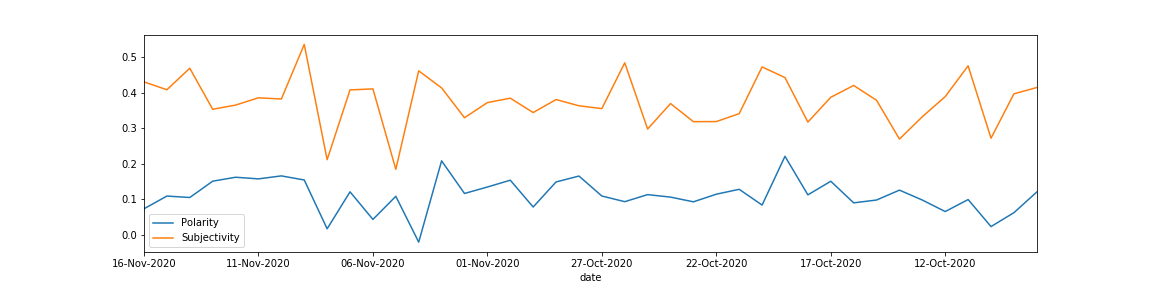
\includegraphics[width=3.0in]{image/sentiment.png}
    \caption{Polarity and Subject in time series}
    \label{top20}
\end{figure}



\end{document}